\section{Statistisk inferens}
I dette afsnit vil vi udføre inferens omkring


\subsection{Bootstrap}
På figur \ref{fig:bootstrap_lasso} ses bootstrap resultater af variable valgt af lasso udfra krydsvalidering.

Flere variable har koefficienter meget tæt på nul og 
variabler \texttt{CE16OV} og \texttt{CLF16OV} .
Dette kan bekræftes af figuren til højre, hvor vi ser, at \texttt{lag1}, \texttt{UEMP150V}, \texttt{UEMP5TO14}, \texttt{UEMPLT5}, \texttt{CE16OV} og \texttt{CLF16OV} lader til at være variablerne som vælges ofte af lasso.
%
\begin{figure}[h]
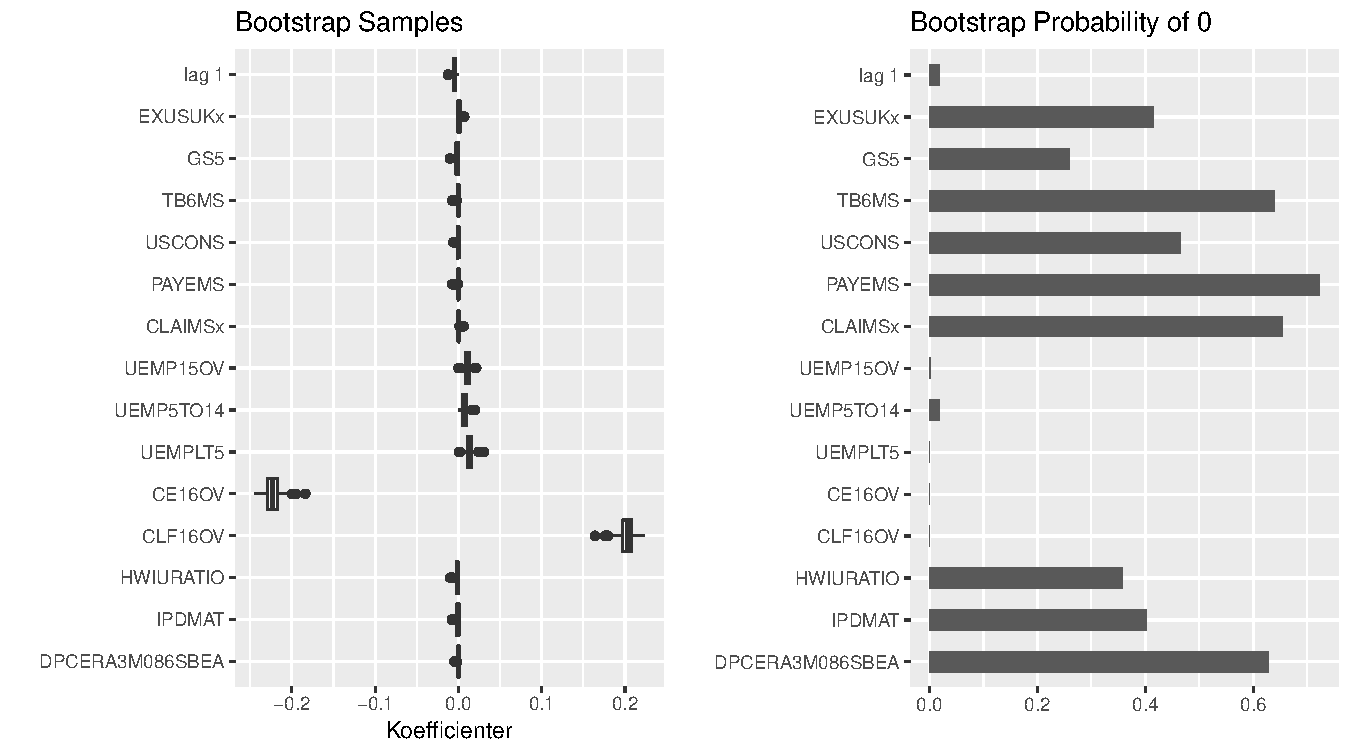
\includegraphics[scale=0.8, clip, trim=0 2.5cm 0 0]{fig/img/bootstrap_lasso.pdf}
\caption{Til venstre ses et boxplot af 1000 bootstrap realisationer af \(\widehat{\tbeta}^\text{lasso} \del{\widehat{\lambda}_\text{CV}}\), mens plottet til højre figur illustrerer andelen af bootstrap realisationer hvor parameter estimaterne er præcis lig nul.}
\label{fig:bootstrap_lasso}
\end{figure}
%
%\fbox{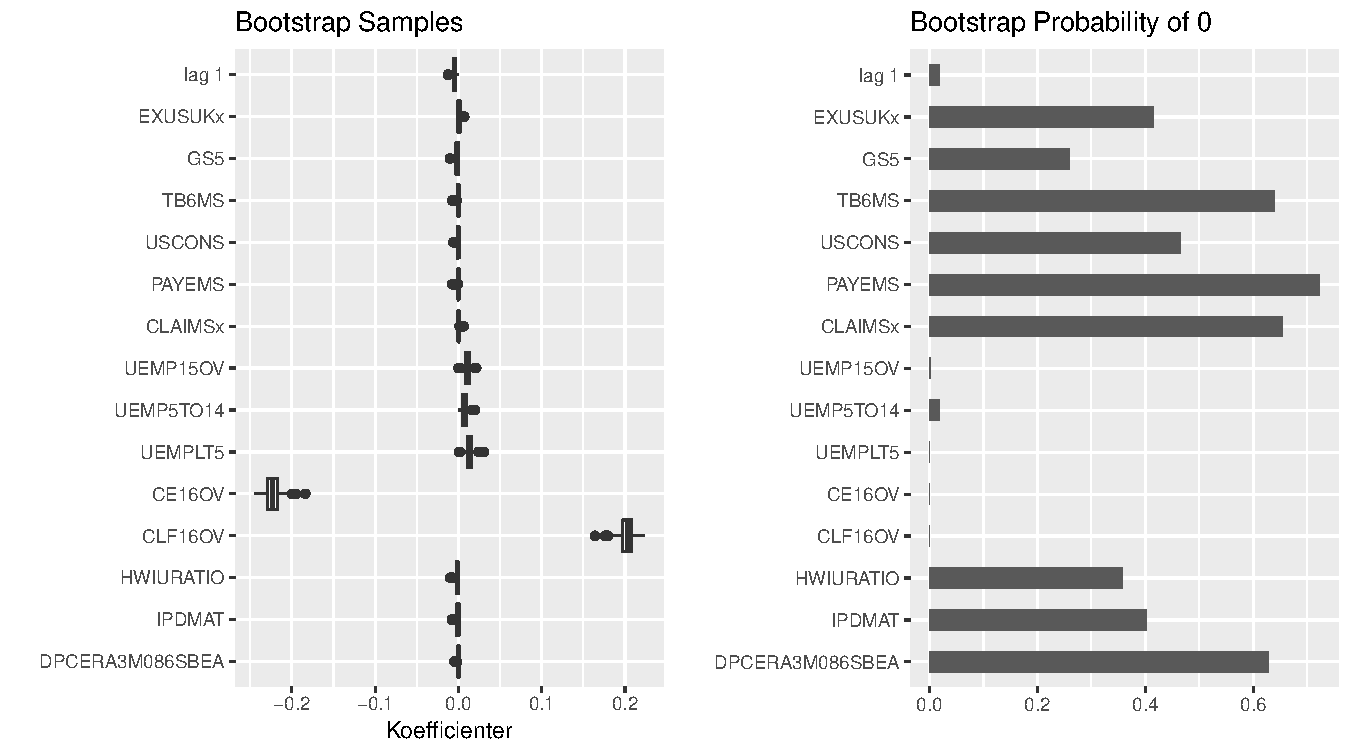
\includegraphics[scale=0.8, trim=0 2.5cm 0 0]{fig/img/bootstrap_lasso.pdf}}



%
%\imgfigh{bootstrap_alassoOLS.pdf}{1}{-.}{Bootstrap_alasso_OLS}
%
%\imgfigh{bootstrap_alassoRidge.pdf}{1}{-.}{bootstrap_alassoRidge}
%
%\imgfigh{bootstrap_grouplasso.pdf}{1}{-.}{bootstrap_grouplasso}
%
%\imgfigh{bootstrap_EN.pdf}{1}{-.}{bootstrap_EN}




\newpage
\subsection{Kovarians test}
Som nævnt udfører LARS med lasso modifikationen 192 steps, hvori variablerne tilføjes og nogle fjernes igen.

Kovarians testen gentager LARS med lasso modifikation og tester nulhypotesen om 

Tildeler \(p\)-værdier til hver variablen som variablen tilføjes til modellen.


Af tabel \ref{tab:covTest} ses, at for prædiktor \texttt{UEMP15OV} (27), \texttt{UEMPLT5} (25), \texttt{CE16OV} (23) og \texttt{CLF16OV} (22) afvises nulhypotesen.
\begin{table}[ht] 
\centering 
\begin{tabular}{llll}
\multicolumn{4}{c}{Lasso} \\
\toprule
Step & Prædiktor & Cov test & \(p\)-værdi \\
\midrule
1 & 27 &  168.9427 & 0.0000 \\
2 & 25 & 168.9155 & 0.0000 \\
3 & 23 &  15.2781 & 0.0000 \\
4 & 22 & 256.4977 & 0.0000 \\
5 & 80 & 0.3717 & 0.6898 \\
6 & 123 & 0.3868 & 0.6795 \\
7 & 78 & 0.0508 & 0.9505 \\
8 & 34 & 0.2940 & 0.7454 \\
9 & 3 & 0.2595 & 0.7715 \\
10 & 94 & 0.0503 & 0.9509 \\
11 & 30 & 0.0705 & 0.9320 \\
12 & 126 & 0.1462 & 0.8641 \\
13 & 105 & 0.0191 & 0.9811 \\
14 & 57 & 0.0042 & 0.9958 \\
15 & 40 & 0.0197 & 0.9805 \\
16 & 24 & 0.0505 & 0.9508 \\
17 & 51 & 0.0085 & 0.9915 \\
18 & 15 & 0.0425 & 0.9584 \\
19 & 93 & 0.0832 & 0.9201 \\
20 & 69 & 0.0377 & 0.9630 \\
21 & 98 & 0.0082 & 0.9918 \\
22 & 101 & 0.0038 & 0.9962 \\
23 & 33 & 0.0115 & 0.9885 \\
24 & 58 & 0.0217 & 0.9786 \\
25 & 2 & 0.0019 & 0.9981 \\
26 & 124 & 0.3875 & 0.6790 \\
27 & 37 & 0.0448 & 0.9562 \\
28 & 103 & 0.0378 & 0.9629 \\
29 & 5 & 0.0125 & 0.9876 \\
30 & 119 & 0.0127 & 0.9873 \\
31 & 73 & 0.0028 & 0.9972 \\
32 & 39 & 0.0539 & 0.9476 \\
33 & 41 & 0.0185 & 0.9817 \\
34 & 17 & 0.0011 &0.9989 \\
35 & 68 & 0.0051 & 0.9949 \\
36 & 72 & 0.1267 & 0.8810 \\
37 & 113 & 0.0009 & 0.9991 \\
38 & 9 & 0.0501 & 0.9511 \\
39 & 54 & 0.0032 & 0.9968 \\
40 & 125 & 0.0049 & 0.9951 \\
%               60             0.0099  0.9902
%              118             0.0022  0.9978
%               84             0.0035  0.9965
%               46             0.0412  0.9596
%              114             0.0151  0.9850
%                7             0.0010  0.9990
%               42             0.0058  0.9942
%               10             0.0043  0.9957
%               56             0.0046  0.9955
%              100             0.0022  0.9978
%               87             0.0001  0.9999
%               67             0.0079  0.9921
%              121             0.0043  0.9957
%              115             0.0046  0.9954
%                4             0.0036  0.9964
%               91             0.0238  0.9764
%              107             0.0280  0.9724
%              111             0.0006  0.9994
%               48             0.0010  0.9990
%              110             0.0152  0.9849
%               85             0.0054  0.9946
%               59             0.0004  0.9996
%               21             0.0029  0.9971
%               81             0.0184  0.9818
%               92             0.0016  0.9984
%              117             0.0026  0.9974
%              116             0.0420  0.9589
%               62             0.0073  0.9927
%               97             0.0176  0.9826
%               19             0.0037  0.9963
%               77             0.0317  0.9688
%               45             0.0094  0.9907
%               99             0.0068  0.9932
%              102             0.0799  0.9232
%               65             0.0036  0.9964
%              120             0.0010  0.9990
%               95             0.0000  1.0000
%               26             0.0248  0.9755
%               83             0.0028  0.9972
%               63             0.0033  0.9967
%               36             0.0077  0.9923
%               31             0.0003  0.9997
%               49             0.0568  0.9448
%                6             0.0056  0.9944
%               55             0.0000  1.0000
%               79             0.0124  0.9877
%               28             0.0065  0.9936
%               43             0.0002  0.9998
%               89             0.0333  0.9673
%               96             0.0214  0.9788
%               12             0.0019  0.9981
%              109             0.0206  0.9796
%               53             0.0008  0.9992
%               86             0.0002  0.9998
%               20             0.0118  0.9883
%               18             0.0002  0.9998
\bottomrule
\end{tabular}  
\caption{lasso \(p\)-værdier.
Tallene er afrundet til 3 decimaler.
Vi viser kun \(p\)-værdier for steps for hvilket en prædiktor medtages og bliver i modellen resten af stien, dvs hvis en prædiktor medtages i et step og senere forlader, vises denne prædiktor ikke.}
\end{table} 



\newpage
\subsection{Teste baseret på polyhedral lemmaet}

Da antallet af parametre er mindre end antallet af observationer i træningsmængden, kan \(\sigma^2\) estimeres udfra SSR fra den fulde model med alle prædiktorer.
Vi finder, at \(\widehat{\sigma} \approx 0.0433\).

Tuning parameteren \(\lambda\) vælges udfra krydsvalidering, som vi fandt \(\lambda \approx 0.0033\), hvorfra lasso valgte 14 variable.




Post-selection intervallerne vises på figur -- for disse 14 variable.


\texttt{fixedLassoInf} udregner \(p\)-værdier og konfidens intervaller for lasso estimatet for en fast værdi af tuning parameteren \(\lambda\).
\texttt{fixedLassoInf} anvender ``standard'' lasso
\begin{align*}
\frac{1}{2} \Vert \y - \X \tbeta \Vert_2^2 + \lambda \Vert \tbeta \Vert_1.
\end{align*}
\texttt{glmnet} multiplicerer først led med faktoren \(\frac{1}{n}\).
Efter vi har kørt \texttt{glmnet} og fundet betaen som svarer til lambda værdien, da skal vi \texttt{beta = coef(obj, s=lambda/n)}, hvor \texttt{obj} er objektet som er returneret af \texttt{glmnet}.


Af figur \ref{fig:fixedLassoInf} observeres at nulhypotesen afvises for \texttt{CLF16OV}, \texttt{CE16OV} samt \texttt{lag 1}.

\begin{table}[h] 
\centering 
\scalebox{0.8}{
\begin{tabular}{llllllll}
\toprule
Prædiktor & Koefficient & Z-score & \(p\)-værdi & lowConfPt & UpConfPt & LowTailArea & UpTailArea\\
\midrule
\textcolor{red3}{DPCERA3M086SBEA} & -0.002 & -1.365 &  0.666  &  -0.009  &  0.026   &    0.050   &   0.050 \\
\textcolor{chartreuse4}{IPDMAT} & -0.003  &-1.113  & 0.268  &  -0.012 &   0.006    &   0.050    &  0.049 \\
\textcolor{blue3}{HWIURATIO}  & 0.002 &  0.718 &  0.197 &   -0.003 &   0.014  &     0.049  &    0.050 \\
\textcolor{blue3}{CLF16OV} & 0.243 & 36.668  & 0.000   &  0.232  &  0.259     &  0.049  &    0.049 \\
\textcolor{blue3}{CE16OV} &  -0.266 & -37.390 &  0.000  &  -0.280 &  -0.254   &    0.049  &    0.049\\
\textcolor{blue3}{UEMPLT5} & 0.001  & 0.241  & 0.402  &  -0.005  &  0.008     &  0.049   &   0.049\\
\textcolor{blue3}{UEMP5TO14} & 0.000 & -0.118 &  0.429  &  -0.007  &  0.004   &    0.049  &    0.049\\
\textcolor{blue3}{UEMP15OV}& 0.004  & 1.593  & 0.056 &    0.000  &  0.009  &     0.049    &  0.050 \\
\textcolor{blue3}{PAYEMS} & 0.001 &  0.273  & 0.223  &  -0.007  &  0.029     &  0.050   &   0.050 \\
\textcolor{blue3}{USCONS} & -0.002 & -0.883 &  0.569 &   -0.009  &  0.016  &     0.050  &    0.000 \\
\textcolor{orange}{TB6MS} & -0.001 & -0.480 &  0.682 &   -0.009  &  0.026  &     0.050   &   0.050 \\
\textcolor{orange}{GS5} & -0.003 & -1.131  & 0.219  &  -0.025  &  0.007     &  0.050   &   0.049\\
\textcolor{orange}{EXUSUKx} & 0.003 &  1.306 &  0.872 &   -0.072  &  0.003  &     0.050  &    0.050 \\
\textcolor{blue3}{lag 1} & -0.009 & -4.067  & 0.003 &   -0.013 &  -0.004  &     0.049    &  0.049 \\
\bottomrule
\end{tabular}  
}
\caption{\(p\)-værdier og konfidensintervaller for variablerne udvalgt af lasso. Den estimeres standard afvigelse er \(0.043\), og resultaterne er for \(\lambda \approx 1.823\) med \(\alpha = 0.1\).} \label{fig:fixedLassoInf}
\end{table} 
